% Written by make_results.py from wave3_heldout_20261025T1625Z/<suite>/report/metrics.json. Do not edit.
% Runs that met the case's outcome, per policy and suite (held-out, one run of the protocol).
\documentclass[border=4pt]{standalone}
% Shared preamble of the older standalone TikZ figures that the documentation still uses
% (fig_roles, fig_loop, fig_freeze, fig_failure, fig_qr). It loads the Plan B figure style and maps
% the older colour and box names onto it: flat white boxes, thin rules, 1 pt corners, no pastel
% fills. New figures input planb_figstyle.tex directly.
% Shared style of every Plan B figure (the deck, the poster and the documentation).
% Type is near-black and grey on white. UMB blue is the brand and the system. One warm accent
% marks tension only (the incoming message, the clock). Green marks only an accepted receipt or
% a met run. Square corners, thin rules, no shadows, no gradients.
\usepackage[T1]{fontenc}
\usepackage[scaled]{helvet}
\renewcommand{\familydefault}{\sfdefault}
\usepackage{tikz}
\usepackage{pgfplots}
\pgfplotsset{compat=1.18}
\usepackage{fontawesome5}
\hyphenpenalty=10000
\exhyphenpenalty=10000
\usetikzlibrary{arrows.meta,positioning,calc,fit,backgrounds}

% Colours
\definecolor{primary}{HTML}{08457E}   % UMB blue: the system, Plan B's own policy
\definecolor{primarysoft}{HTML}{E7EEF5}
\definecolor{accent}{HTML}{FF791F}    % tension only: the message, the gap, the one missed run
\definecolor{accentsoft}{HTML}{FFEBDC}
\definecolor{umbblue}{HTML}{005A8B}   % UMB blue: the three idea marks and structure
\definecolor{navy}{HTML}{132245}      % title bands, the receipt, the dark close
\definecolor{ground}{HTML}{EEF2F6}    % the light blue-grey ground behind white cards
\definecolor{ok}{HTML}{2E7D32}        % an accepted receipt, a met run
\definecolor{oksoft}{HTML}{E5F1E6}
\definecolor{ink}{HTML}{1F1F1F}
\definecolor{muted}{HTML}{6B6B6B}
\definecolor{quiet}{HTML}{9A9A9A}     % other policies, context
\definecolor{rulegrey}{HTML}{C4C4C4}
\definecolor{gridgrey}{HTML}{E4E4E4}
\definecolor{faint}{HTML}{F4F4F4}

\tikzset{
  >={Stealth[length=2.4mm,width=1.8mm]},
  every picture/.style={line cap=butt, line join=miter},
  % text styles
  hd/.style={font=\bfseries, text=ink, align=left},
  sub/.style={text=muted, align=left},
  % shapes: square or 1 pt corners, thin rules
  card/.style={draw=rulegrey, line width=0.5pt, fill=white, rounded corners=1pt, inner sep=5pt, align=left, text=ink},
  sys/.style={draw=primary, line width=0.8pt, fill=white, rounded corners=1pt, inner sep=5pt, align=center, text=ink},
  sysfill/.style={draw=primary, line width=0.8pt, fill=primary, rounded corners=1pt, inner sep=5pt, align=center, text=white},
  warm/.style={draw=accent, line width=0.8pt, fill=accentsoft, rounded corners=1pt, inner sep=5pt, align=left, text=ink},
  receipt/.style={draw=ok, line width=0.8pt, fill=oksoft, rounded corners=1pt, inner sep=5pt, align=left, text=ink},
  planned/.style={draw=muted, line width=0.6pt, dash pattern=on 3pt off 2pt, fill=white, rounded corners=1pt, inner sep=5pt, align=left, text=muted},
  % connectors
  link/.style={->, draw=muted, line width=0.6pt},
  syslink/.style={->, draw=primary, line width=0.9pt},
  oklink/.style={->, draw=ok, line width=0.9pt},
  warmlink/.style={->, draw=accent, line width=0.9pt},
  nextlink/.style={->, draw=muted, line width=0.6pt, dash pattern=on 3pt off 2pt},
}

% Charts: a real axis, few light gridlines, no frame on the top and right.
\pgfplotsset{
  planb/.style={
    axis line style={draw=muted, line width=0.5pt},
    tick style={draw=muted, line width=0.5pt},
    major tick length=3pt,
    tick label style={text=ink, /pgf/number format/assume math mode=true},
    label style={text=ink},
    title style={font=\bfseries, text=ink},
    grid style={draw=gridgrey, line width=0.4pt},
    every axis plot/.append style={line width=0.6pt},
    legend style={draw=none, fill=none, text=ink},
    legend cell align=left,
  },
}

% The three idea marks, the same in the deck, the poster and the report.
% 1 Check the fact (a magnifier), 2 Pick only what fits (a funnel that keeps what fits),
% 3 Leave a receipt (a receipt slip). Always in UMB blue unless the panel is navy.
\providecommand{\markcheck}{\faSearch}
\providecommand{\markfits}{\faFilter}
\providecommand{\markreceipt}{\faReceipt}
% The three points of "Why Plan B": safer shows the three marks together, more flexible a laptop,
% more personal a set of sliders.
\providecommand{\marksafer}{\faSearch\,\faFilter\,\faReceipt}
\providecommand{\markflexible}{\faLaptop}
\providecommand{\markpersonal}{\faSlidersH}

\usetikzlibrary{shapes.geometric,patterns}

\colorlet{umbdark}{ink}
\colorlet{umbblue}{primary}
\colorlet{umborange}{accent}
\definecolor{umbyellow}{HTML}{FEDE42}
\colorlet{line}{rulegrey}
\colorlet{okgreen}{ok}
\colorlet{softblue}{white}
\colorlet{softorange}{white}
\colorlet{softgreen}{white}
\colorlet{softgray}{faint}

\tikzset{
  flow/.style={->, draw=muted, line width=0.6pt},
  box/.style={draw=rulegrey, line width=0.5pt, fill=white, rounded corners=1pt, align=center, inner sep=5pt, text=ink},
  keybox/.style={draw=primary, fill=white, rounded corners=1pt, align=center, inner sep=5pt, text=ink, line width=0.8pt},
  hotbox/.style={draw=accent, fill=white, rounded corners=1pt, align=center, inner sep=5pt, text=ink, line width=0.8pt},
  okbox/.style={draw=ok, fill=white, rounded corners=1pt, align=center, inner sep=5pt, text=ink, line width=0.8pt},
  lbl/.style={text=muted, align=center},
}

\begin{document}
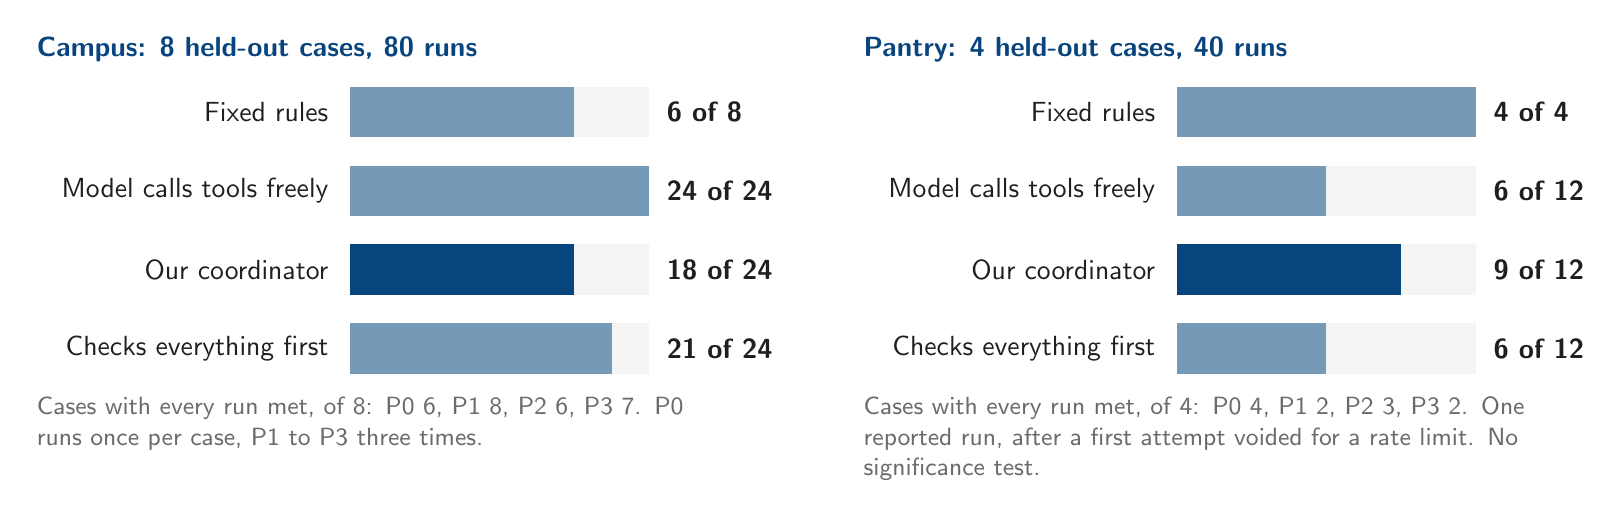
\begin{tikzpicture}[font=\normalsize]
\node[anchor=west, font=\bfseries\color{primary}] at (-4.10,0.80) {Campus: 8 held-out cases, 80 runs};
\node[anchor=east, text=ink] at (-0.15,0.00) {Fixed rules};
\fill[softgray] (0.00,-0.32) rectangle (3.80,0.32);
\fill[umbblue!55] (0.00,-0.32) rectangle (2.850,0.32);
\node[anchor=west, text=ink] at (3.90,0.00) {\bfseries 6 of 8};
\node[anchor=east, text=ink] at (-0.15,-1.00) {Model calls tools freely};
\fill[softgray] (0.00,-1.32) rectangle (3.80,-0.68);
\fill[umbblue!55] (0.00,-1.32) rectangle (3.800,-0.68);
\node[anchor=west, text=ink] at (3.90,-1.00) {\bfseries 24 of 24};
\node[anchor=east, text=ink] at (-0.15,-2.00) {Our coordinator};
\fill[softgray] (0.00,-2.32) rectangle (3.80,-1.68);
\fill[primary] (0.00,-2.32) rectangle (2.850,-1.68);
\node[anchor=west, text=ink] at (3.90,-2.00) {\bfseries 18 of 24};
\node[anchor=east, text=ink] at (-0.15,-3.00) {Checks everything first};
\fill[softgray] (0.00,-3.32) rectangle (3.80,-2.68);
\fill[umbblue!55] (0.00,-3.32) rectangle (3.325,-2.68);
\node[anchor=west, text=ink] at (3.90,-3.00) {\bfseries 21 of 24};
\node[anchor=north west, text=muted, font=\small, align=left, text width=8.8cm] at (-4.10,-3.50) {Cases with every run met, of 8: P0 6, P1 8, P2 6, P3 7. P0 runs once per case, P1 to P3 three times.};
\node[anchor=west, font=\bfseries\color{primary}] at (6.40,0.80) {Pantry: 4 held-out cases, 40 runs};
\node[anchor=east, text=ink] at (10.35,0.00) {Fixed rules};
\fill[softgray] (10.50,-0.32) rectangle (14.30,0.32);
\fill[umbblue!55] (10.50,-0.32) rectangle (14.300,0.32);
\node[anchor=west, text=ink] at (14.40,0.00) {\bfseries 4 of 4};
\node[anchor=east, text=ink] at (10.35,-1.00) {Model calls tools freely};
\fill[softgray] (10.50,-1.32) rectangle (14.30,-0.68);
\fill[umbblue!55] (10.50,-1.32) rectangle (12.400,-0.68);
\node[anchor=west, text=ink] at (14.40,-1.00) {\bfseries 6 of 12};
\node[anchor=east, text=ink] at (10.35,-2.00) {Our coordinator};
\fill[softgray] (10.50,-2.32) rectangle (14.30,-1.68);
\fill[primary] (10.50,-2.32) rectangle (13.350,-1.68);
\node[anchor=west, text=ink] at (14.40,-2.00) {\bfseries 9 of 12};
\node[anchor=east, text=ink] at (10.35,-3.00) {Checks everything first};
\fill[softgray] (10.50,-3.32) rectangle (14.30,-2.68);
\fill[umbblue!55] (10.50,-3.32) rectangle (12.400,-2.68);
\node[anchor=west, text=ink] at (14.40,-3.00) {\bfseries 6 of 12};
\node[anchor=north west, text=muted, font=\small, align=left, text width=8.8cm] at (6.40,-3.50) {Cases with every run met, of 4: P0 4, P1 2, P2 3, P3 2. One reported run, after a first attempt voided for a rate limit. No significance test.};
\end{tikzpicture}
\end{document}
